\chapter{Revisão Bibliográfica} \label{cap:rev}
\section{Fundamentação teórica} 


Várias empresas aproveitam a crescente acessibilidade da população a dispositivos móveis, para criar e disponibilizar produtos em lojas virtuais como Apple Store e Play Store.

Com esta grande popularização, muitas destas empresas utilizam-se de frotas de entregadores e fornecedores autônomos, sem ter a necessidade de gastar com veículo ou produto. Como exemplos, há os casos do Uber, empresa voltada a transporte pessoal similar ao sistema de Táxi; Airbnb, uma empresa voltada a gerenciar locais como pousadas, hotelarias ou aluguel residencial sem ter qualquer imóvel; Ifood, um dos grandes nomes de entrega de comidas existentes sem ter seu restaurante próprio.

Mas a utilização desses aplicativos, além de possibilitar que o motorista seja autônomo, também traz grandes problemas. A utilização dos \textit{smartphones} na condução é responsável por  mais de 150 mortes diariamente, envolvendo todas as modalidades veiculares. Uma pesquisa realizada pela Associação Brasileira de Medicina de Trânsito (ABRAMET) indica que a atenção requerida para a utilização dos \textit{smartphones} aumenta em até 4 vezes o risco de acidentes, inclusive na utilização do viva-voz. Na realização de uma chamada simples, o condutor utiliza, em média, 5 segundos para digitar o telefone. Este tempo é mais que suficiente para que acidentes sejam causados ou sofridos.

Como destaca Diogo Garcia, cirurgião e especialista da Emergência Especializada em Trauma do Hospital Samaritano de São Paulo, a primeira hora para a realização dos primeiros socorros é vital para a sobrevivência e redução de sequelas das vítimas de acidente. Do total de fatalidades em acidentes de trânsito, 35\% ocorrem entre 1 e 4 horas após o trauma, sendo o período crítico compreendido de uma hora entre o acidente, transporte e tratamento adequado conhecido como \textit{“golden hour”}.

\begin{citacao}

        "Nesse período de uma hora, o atendimento ao traumatizado deve ser realizado por uma equipe multiprofissional e altamente especializada para evitar complicações como sequelas graves e até mesmo a morte. O atendimento é baseado em protocolos médicos internacionais que garantem o tratamento das lesões por ordem de gravidade" \cite{lio2019atendimento}. \par

\end{citacao}

    




Dessa forma faz-se necessário que o atendimento seja efetuado o mais rápido possível, sendo a rapidez no acionamento do serviço emergencial um grande destaque. Nos casos em que o \textit{motoboy} sofre de graves sequelas ou longos períodos de  recuperação, o mesmo pode recorrer aos seguros de vida  e até mesmo a previdência. 
Os seguros de vida existentes, em sua grande maioria, não cobrem os lucros cessantes, somente o prêmio de acordo com o contrato e as perdas, ou seja, apenas seria compensado pelos danos físicos sofridos e não teria o acréscimo dos dias que não pode trabalhar. Nesse segundo caso o \textit{motoboy} deveria recorrer ao sistema de previdência. 

Como o "\textit{motoboy} de aplicativo" não é um funcionário com carteira registrada, o mesmo não possui qualquer tipo de auxílio a não ser que esteja contribuindo com o Instituto Nacional do Seguro Social (INSS) ou qualquer outro sistema de previdência privada, porém as previdências privadas, em geral, são voltadas para as poupanças a longo prazo e não de seguridade. 
Há a existência de um Projeto de Lei (pl 6789 da Câmara dos Deputados), não aprovado até o momento, que prevê a obrigatoriedade do seguro de vida para \textit{motoboys} e entregadores. Tal obrigatoriedade prevista é de difícil fiscalização para os aplicativos de \textit{delivery} tendo em vista que não há contrato entre o motorista e o aplicativo. Também não tem como responsabilizar o aplicativo pois ele não está constantemente com os entregadores, assim como as empresas que o utilizam já que não possuem qualquer vínculo trabalhista. 

Nessas condições para o \textit{motoboy} é extremamente desvantajoso permanecer parado. Nos casos de ser extremamente necessário, como no caso dos acidentes, que esse tempo seja o mais breve possível. 

Nesta seção serão discutidos os benefícios na utilização dos aplicativos de \textit{delivery}, seus riscos e uma visão geral do mercado.

\subsection{\textbf{Mercado em crescimento}}
De acordo com a notícia escrita  do jornal O Globo, o setor de transporte gerou 133 mil vagas em fevereiro graças a utilização dos aplicativos móveis, pois basta o usuário  ter um veículo para se locomover e ser apto a realizar entregas. Segundo os dados adquiridos pelo autor  através da CNC (Confederação Nacional do Comércio) entre os anos de 2008 e 2018 houve um crescimento de 74\% somente no número de motociclistas no Rio de Janeiro
\cite{costa2019s}.
\subsection{\textbf{Riscos}}

A quantidade de acidentes fatais sofridos por motociclistas aumentou 17,7\% em 2018 com relação a 2017 na cidade de São Paulo, chegando a uma média de pelo menos uma morte por dia. Destaca-se, também, o fato de que os aplicativos de entregas dão bônus em dinheiro para aqueles que fazem mais entregas em menor espaço de tempo \cite{2019acidentes}.

O Estadão de São Paulo  cita o aumento de aproximadamente 18\% de acidentes com motociclistas devido a utilização dos aplicativos de entregas, a matéria possui um mapa contendo todos os pontos de acidentes ocorridos em 2017 e 2018, mostrado na Figura 1 \cite{ribeiro2019mortes}.



 \begin{figure}[H]

 \caption{Mapa contendo todos os pontos de mortes registradas por motociclistas}
  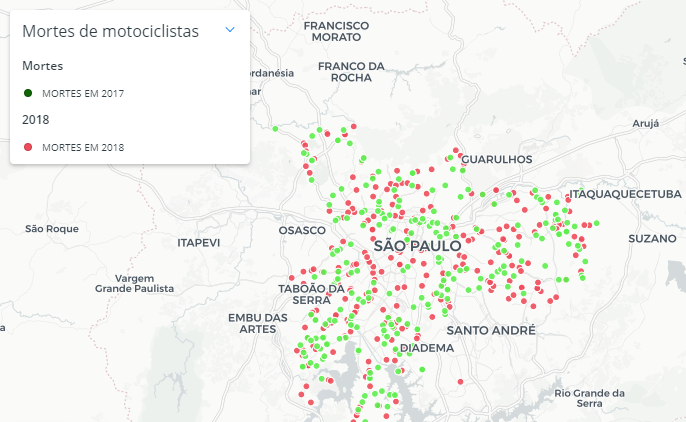
\includegraphics[width=\textwidth]{images/Cap2/mapa.png}
   \scriptsize  Fonte : Ribeiro e Felix 2019
   
  \end{figure}

Também é destacado o estímulo exagerado por estes aplicativos de entregas que incentivam os motociclistas a saírem para realizar suas entregas mesmo em condições desfavoráveis, oferecendo uma comissão por realizar suas entregas  em dias chuvosos como é demonstrado na Figura 2, que contém mensagens de SMS de alguns aplicativos de \textit{delivery} conhecidos atualmente.



 \begin{figure}[H] 

 \caption{Mensagens de incentivos recebidas por motociclistas}
  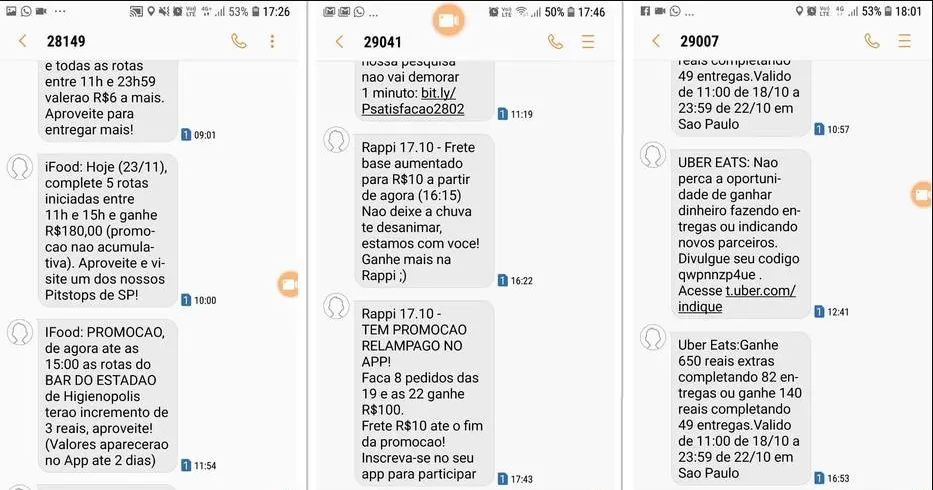
\includegraphics[width=\textwidth]{images/Cap2/whtas.png}

 \scriptsize  Fonte : Ribeiro e Felix 2019 
  
\end{figure}



\section{Trabalhos correlatos}


\subsection{\textbf{Estudo da dinâmica das motocicletas em frenagens e curvas}}


 O estudo da dinâmica das motocicletas em frenagens e curvas com o efeito da técnica do piloto e da condição da estrada, a técnica do piloto nas mais adversas situações é determinante para manter-se sob controle em situações de risco. Nesse estudo, os autores objetivaram determinar a velocidade máxima para a realização de curvas previamente determinadas e quando o piloto deve iniciar a frenagem a fim de evitar acidentes.\cite{Magnani2017Saulo}

O estudo envolveu a análise de diversas forças que atuam sobre o veículo, como a força aplicada na roda traseira, a força normal de ambas as rodas e a força de frenagem em ambas as rodas que depende do coeficiente de utilização do freio.  As forças que tendem a resistir ao movimento da motocicleta são correspondentes à resistência aerodinâmica (Fa), resistência à deformação dos pneus (Fr,t), e o componente gravitacional em direção do movimento(Fg). Todas as forças citadas estão representadas na Figura 3.




    
 \begin{figure}[H] 

 \caption{Forças existentes no movimento e frenagem da motocicleta}

  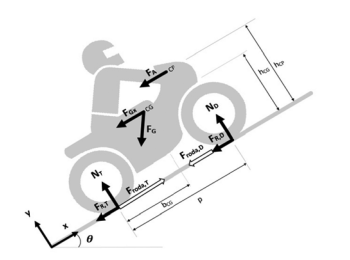
\includegraphics[width=150mm]{images/Cap2/forca.png}

    \scriptsize  Fonte : Maganani e Cunha 2017
  \end{figure}

    

 
  
  Em sua conclusão, os autores identificaram que a desaceleração é altamente dependente do coeficiente de atrito em cada situação, de forma a não recomendar uma técnica universal de frenagem. Os cenários de desaceleração em reta, curvas e desaceleração em curvas estudados foram elevados ao limite, estes cenários atingidos apenas por pilotos profissionais é raramente visto cotidianamente. 

Neste estudo se destacam as informações de ângulo máximo das motocicletas comerciais limitado pelo conjunto da pedaleira que fica em aproximadamente 50º e a força de desaceleração máxima atingida em uma forte redução de velocidade de 100km/h a 60km/h, chegando até 1.05g, de forma a auxiliar no reconhecimento de possíveis acidentes. 




\subsection{\textbf{Monitoramento da agressividade na direção}}


O monitoramento da agressividade na direção de caminhões através de acelerômetro e GPS  utiliza um sistema embarcado composto por um microcontrolador, acelerômetro, GPS e GSM para monitorar as ações dos motoristas de caminhões, determinando se o comportamento ao dirigir é perigoso e sinalizando tal comportamento por e-mail. Os dados obtidos pelo sistema embarcado são enviados para um servidor que compila e mostra a trajetória do motorista, bem como os trechos nos quais houve agressividade em sua condução como demonstra a Figura 3.



 \begin{figure}[H]

 \caption{Tela de análise da viagem}

  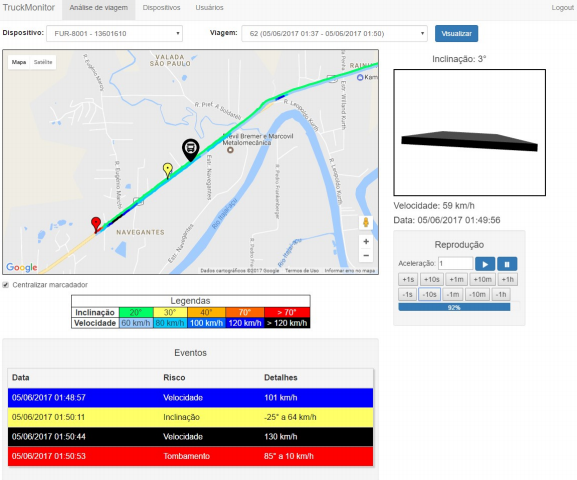
\includegraphics[width=150mm]{images/Cap2/analise.png}
  
  \scriptsize Fonte: Schlag 2017
\end{figure}

  
      




O dispositivo de aquisição é composto por um microcontrolador ESP modelo 8266, um módulo contendo acelerômetro e giroscópio sendo este o MPU-6560 e um módulo GPS/GSM para localização e envio dos dados. 

Os testes do sistema foram realizados ao longo de 250 quilômetros, em um caminhão modelo Scania P310, envolvendo trechos de rodovias federais e estradas. A velocidade máxima atingida em todo o período chegou a 84 km/h com uma inclinação máxima de 15º. Para avaliar as notificações que necessitam de maiores ângulos, o sistema de aquisição foi rotacionado manualmente.

Neste trabalho, o autor obteve grande assertividade ao detectar excessos de velocidade, conseguindo aferir a mesma com precisão de 4 km/h. Tombamentos e possíveis manobras perigosas também foram registrados. Inclusive as manobras agressivas realizadas para evitar acidentes, nesses casos o dispositivo de aquisição foi movimentado manualmente a fim de evitar manobras arriscadas. 

A precisão obtida pelo autor, que utiliza um dispositivo de aquisição semelhante ao utilizado neste trabalho, é altamente satisfatória o que corrobora com a utilização e escolha do \textit{hardware}.  



\subsection{\textbf{Emprego de giroscópio e acelerômetro na perícia de acidentes}}

A proposta de emprego de giroscópio e acelerômetro na perícia de acidentes automobilísticos propôs um dispositivo embarcado de baixo custo capaz de registrar os dados em acidentes de carro. Em países desenvolvidos, o módulo do sistema de \textit{air bag} também coleta os dados que resultaram em sua ativação. Citando a literatura internacional, os autores buscam algo semelhante à “caixa preta” que é, ou deveria ser no caso de veículos nacionais, o módulo de air bag \cite{lima2016proposta}.

Motivados pelo difícil acesso aos scanners exclusivos dos fabricantes dos veículos e/ou módulos de air bag, buscaram capturar e analisar os dados de segundos antes e após o acidente, de forma a auxiliar no estudo criminalístico. 

Utilizando um sistema embarcado dotado de acelerômetro e giroscópio, o dispositivo foi capaz de armazenar 10,9 segundos de informações relacionadas ao acidente. Tais informações podem ser exportadas para simuladores 3D capazes de reconstruir virtualmente o acidente, em sua conclusão reforçam a grande aplicabilidade de seu sistema, auxiliando os peritos e experts no assunto. 

A aquisição satisfatória dos dados a partir de um dispositivo embarcado que contém acelerômetro e giroscópio de tal modo a ser utilizado em simuladores justifica a utilização e escolha do \textit{ hardware}.



\subsection{\textbf{Uso de \textit{Smartphones} para monitoramento de ciclistas}}

 O projeto  de uso de \textit{Smartphones} para monitoramento de ciclistas e detecção automática de acidentes foi proposto pelos alunos da Universidade Tecnológica de Chalmers é alertar acidentes de ciclistas utilizando o eCall. eCall é um sistema desenvolvido na Europa capaz de monitorar os veículos na estrada, na ocorrência de alguns acidentes o dispositivo acoplado no veículo faz uma ligação para o número de emergência, além de passar as coordenadas do veículo para as autoridades \cite{2019interoperable}.

Como o sistema de eCall é voltado somente para automóveis foi proposto pelos alunos da universidade de Chalmers na Suécia  implementar o sistema de eCall utilizando  \textit{smartphones} para ciclistas, como demonstrado na Figura 5.  Neste projeto não foi utilizado nenhum \textit{hardware} adicional para a medição dos dados, o \textit{smartphone} não precisou de nenhuma fonte de energia externa, pois o aplicativo desenvolvido era econômico em relação a drenagem da bateria do celular  .




 \begin{figure}[H]

 \caption{Princípio do funcionamento do sistema de eCall para ciclista}
  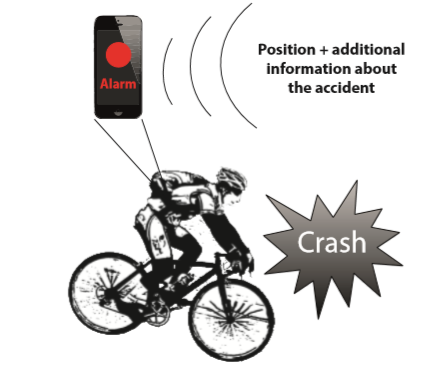
\includegraphics[width=150mm]{images/Cap2/images.png}
 
  \scriptsize Fonte : Candefjord \textit{et al.} 2014
  
\end{figure}

    



Para o monitoramento foram utilizados os seguintes sensores para a medição dos dados, acelerômetro de 3 eixos, sensor de rotação de 3 eixos e sensor de posição GPS com uma taxa de amostragem de 100hz, todos eles já integrados dentro do \textit{smartphones}. Com isto foi possível calcular a aceleração total do ciclista utilizando a equação (2.1).


\begin{equation}
\centering
    \mathit{Acc} = \sqrt{Accx^2 + Accy^2 + Accz^2}
\end{equation}


Para a aquisição dos dados foram registradas mais de 5 horas de dados “normais” onde nenhum acidente ocorreu. Já para os registros de impacto foi utilizado um boneco, que possui as características humanas e um peso de 40kg, que foi submetido a vários testes de queda.

 O gráfico da Figura 6 demonstra uma amostra dos dados coletados. O primeiro intervalo, entre zero e quarenta segundos, representa o ajuste do celular em cima da bicicleta, já o intervalo de noventa e cem segundos mostra um padrão de indicação de acidente.


 \begin{figure}[H]

 \caption{Gráfico dos dados mensuradas}
  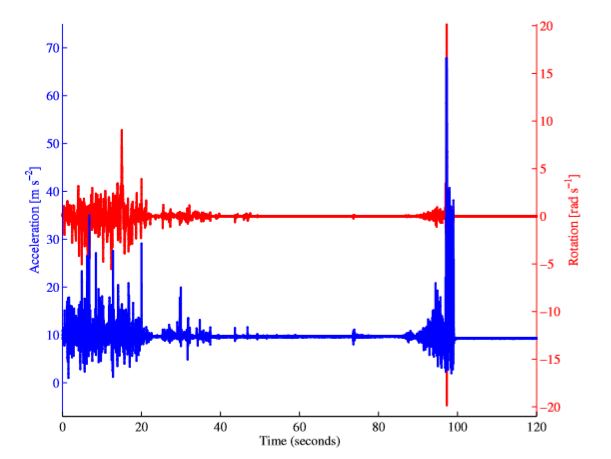
\includegraphics[width=150mm]{images/Cap2/grafico_acelera.png}
 
  \scriptsize Fonte : Candefjord \textit{et al.} 2014
\end{figure}

Analisando este projeto,foi possível perceber que utilizando  somente um \textit{smartphone} para a detecção de uma queda ou acidente, sendo possível disparar sinais de emergência para outros lugares.


\subsection{\textbf{Utilizando \textit{smartphones} como sensor detecção de acidentes de carro}}

O projeto utilizando \textit{smartphones} como sensor móvel sem fio para a detecção de acidentes de carro e providenciar avisos de emergências  foi proposto o desenvolvimento de um aplicativo para \textit{smartphone} responsável por capturar os dados dos sensores de acelerômetro, compasso e GPS, sendo capaz de detectar acidentes e gravar estes dados, como a força G exercida no usuário durante o evento \cite{thompson2010using}.

O sistema foi desenvolvido no formato cliente-Servidor, o \textit{smartphone} envia as informações via internet móvel para o servidor utilizando HTTP post, onde os dados recebidos serão processados e, então, enviará notificações para as autoridades. Na Figura 7 é apresentado o esquemático do sistema criado.

 \begin{figure}[H]

 \caption{Sistema de detecção de acidentes}
  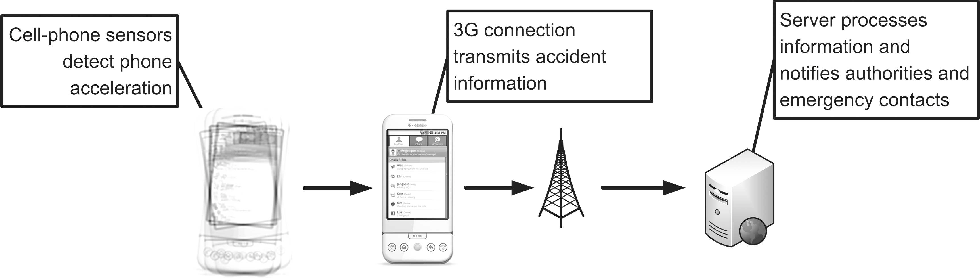
\includegraphics[width=150mm]{images/Cap2/esquema.png}
  
  \scriptsize Fonte: Thompson \textit{et al.} 2010
  
    
\end{figure}



O sistema irá monitorar o comportamento do acelerômetro de três eixos do celular, quando houver uma grande aceleração pelos ocupantes será registrada a força aplicada em relação ao usuário, registrando um evento contendo o valor da força G e a posição do ocorrido, a Figura 8 demonstra quando o aplicativo é acionado.



 \begin{figure}[H]

 \caption{Sistema de detecção de acidentes}
  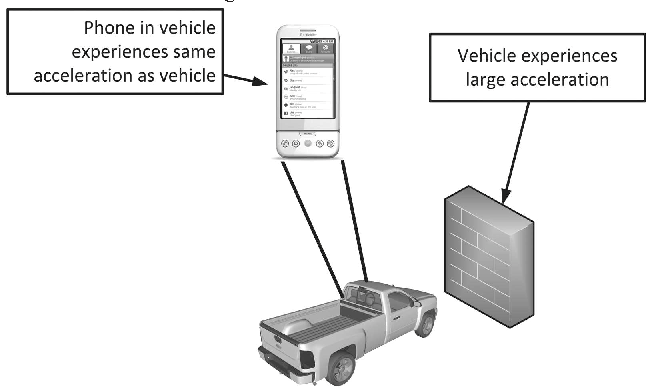
\includegraphics[width=150mm]{images/Cap2/acionamento.png}
  
    \scriptsize Fonte: Thompson \textit{et al.} 2010
\end{figure}



Porém ainda foi necessário verificar os casos falso positivo e removê-los do sistema para que não tenha avisos errados pelo sistema, para isto foram analisados dois casos:

\begin{itemize}
    \item  Filtro de velocidade que determina onde o usuário está no veículo, para prevenir problemas de arranque o aplicativo só começa a medir um potencial acidente a partir de 24 km/h, além disso o sistema fica ativo por 5 minutos mesmo após a desaceleração do veículo, fazendo com que o aplicativo não tenha que ficar recriando sua conexão toda vez que o usuário pare em um semáforo.
\end{itemize}


\begin{itemize}
    \item  Filtro de aceleração que previne paradas bruscas para o acionamento das notificações, para isto o sistema irá ignorar qualquer aceleração bruta menos do que 4G, para isto foram feitos dois testes para determinar estes efeitos, o primeiro foi acelerar o carro até 38 km/h e frear bruscamente gerando o resultado da Figura 9.
    
\end{itemize}


 \begin{figure}[H]

 \caption{Gráfico mostrando os efeitos dos 3 eixos a parada brusca}
  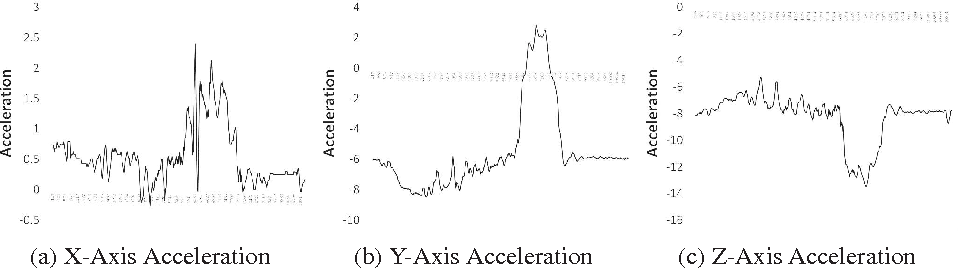
\includegraphics[width=150mm]{images/Cap2/acelerometro_graficos.png}
  
    \scriptsize Fonte: Thompson \textit{et al.} 2010
    
\end{figure}



O segundo teste foi deixar o celular cair em queda livre e verificar os valores do acelerômetro, determinando então que a variação dos acelerômetros foram apenas picos de energia muito rápido registrados como mostra a Figura 10.




 \begin{figure}[H]

 \caption{Gráfico mostrando os 3 eixos do acelerômetro para a queda livre}
  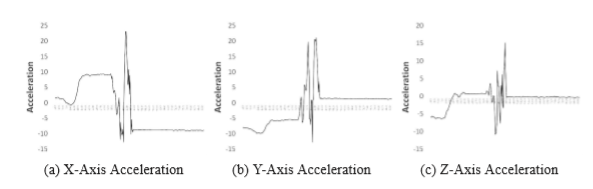
\includegraphics[width=150mm]{images/Cap2/acelerometro_quedalivre.png}
  
    \scriptsize Fonte: Thompson \textit{et al.} 2010
  \end{figure}



Com este projeto foi possível concluir que é viável utilizar um \textit{smartphone} que transmita as informações para um servidor externo pois há uma redução do custo do desenvolvimento e manutenção do serviço, além de não ser necessário a aquisição de um hardware específico.

